\chapter{A visual verification report for ChiselTest}
During F-CSP and Chisel-CRV development, the author carried out a side project
to visually report the coverage metrics collected during testing, including
functional coverage metrics and code coverage metrics collected with the
Verilator~\cite{verilator} backed in ChiselTest.

As stated in the previous chapters, Chisel relies on transforming the
intermediate representation of the FIRRTL stage into Verilog for hardware
synthesis. The Verilog code generated can then be simulated by any Verilog
simulator or directly synthesized by any vendor-specific development tools.

Verilator is an open-source simulator guided by the Chips Alliance and Linux
Foundation project. Verilator allows translating Verilog code to C++/SystemC
code that can be compiled natively and run by any modern computer. Since version
2.1, Verilator started introducing coverage support. The current version of
Verilator (4.108) supports three types of coverage: line coverage, toggle
coverage, and SystemVerilog Assertion property coverage. The recording of the
coverage can be enabled during the translation from Verilog to C++ code by
invoking the Verilator binary with the \textit{--coverage-line},
\textit{--coverage-toggle}, \textit{--coverage-user} parameters, respectively. A
fourth parameter called \textit{--coverage} is available to the users, and it
enables all three types of coverage simultaneously.

The \textit{coverage-line} parameter is used to specify coverage analysis for
each code flow change point in the Verilog source code~\cite{verilatormanual}.
For each of these decision points, a counter is kept and incremented every time
the specific path is taken during the simulation. The \textit{coverage-toggle}
parameter enables the analysis of every signal in a module. With this parameter
enabled, every signal that is not local to the module has a counter that
increments every time the signal changes states. Lastly, the
\textit{coverage-user} parameter enables user-defined functional coverage in the
form of SystemVerilog assertions. This type of coverage is not considered in
this report since it requires manual intervention from the user or implementing
a custom transformation for inserting SystemVerilog assertion in the generated
Verilog code through FIRRTL annotation.

When the simulation is run with coverage enabled, Verilator generates a coverage
report in a SystemPerl~\cite{SystemPerl} coverage report file for each different
test at the end of the simulation. The output of multiple tests can then be
combined by using the \textit{verilator\_coverage} utility provided with
Verilator. The merged report file can then be transformed into an info file and
processed by any coverage tools or extensions.

One of the most used front ends for code coverage is LCOV~\cite{Lcov}. LCOV is a
graphical front end developed as part of the Linux test project, and it can read
coverage results and display them in the form of an HTML page through its
companion utility genhtml. As part of Google Summer Of Code 2014, genhtml was
ported into Java by Rick Brown under the name jgenhtml~\cite{jgenhtml}.

By combining genhtml, Verilator, and ChiselTest, it was possible to
automatically generate a coverage report for each test suite specified inside
ChiselTest. As a part of the research project, it was extended the ChiselTester
library with a custom ScalaTest reporter generator that automatically detects
the coverage files generated by Verilator, merges them, and creates an HTML page
reporting the source code of the module tested and displaying which lines were
covered during the run of the test suite.

Every time the user creates a test suite that mixes a new Scala trait called
CoverageTrait in the ScalaTest suite, a similar output will appear at the end of
the test:
\begin{code}
\begin{minted}
[
frame=lines,
framesep=2mm,
baselinestretch=1.2,
fontsize=\footnotesize,
linenos
]
{bash}
Reading data file: output.info
Found common filename prefix /Users/enrico/Documents/Git/transfer/output/uvm/
Generating output at [...]/transfer/output/uvm/chisel.AluAccuTester
Writing report for AluAccuChisel.v
Writing directory view page.
Overall coverage rate:
	lines......: 100.0% (13 of 13 lines)
	functions: no data found
	branches: no data found
Line coverage 100.0%, 
Coverage saved in file:///[...]/transfer/output/uvm/
chisel.AluAccuTester/VerilatorCoverage.html
[info] ScalaTest
[info] Run completed in 6 seconds, 258 milliseconds.
[info] Total number of tests run: 7
[info] Suites: completed 5, aborted 0
[info] Tests: succeeded 7, failed 0, canceled 0, ignored 0, pending 0
[info] All tests passed.
[info] Passed: Total 7, Failed 0, Errors 0, Passed 7
[success] Total time: 12 s, completed Dec 10, 2020 9:24:46 PM
\end{minted}
\caption{Custom report generator output.}
\label{listing:customhtmlreport}
\end{code}

\begin{figure}[!ht]
\centering
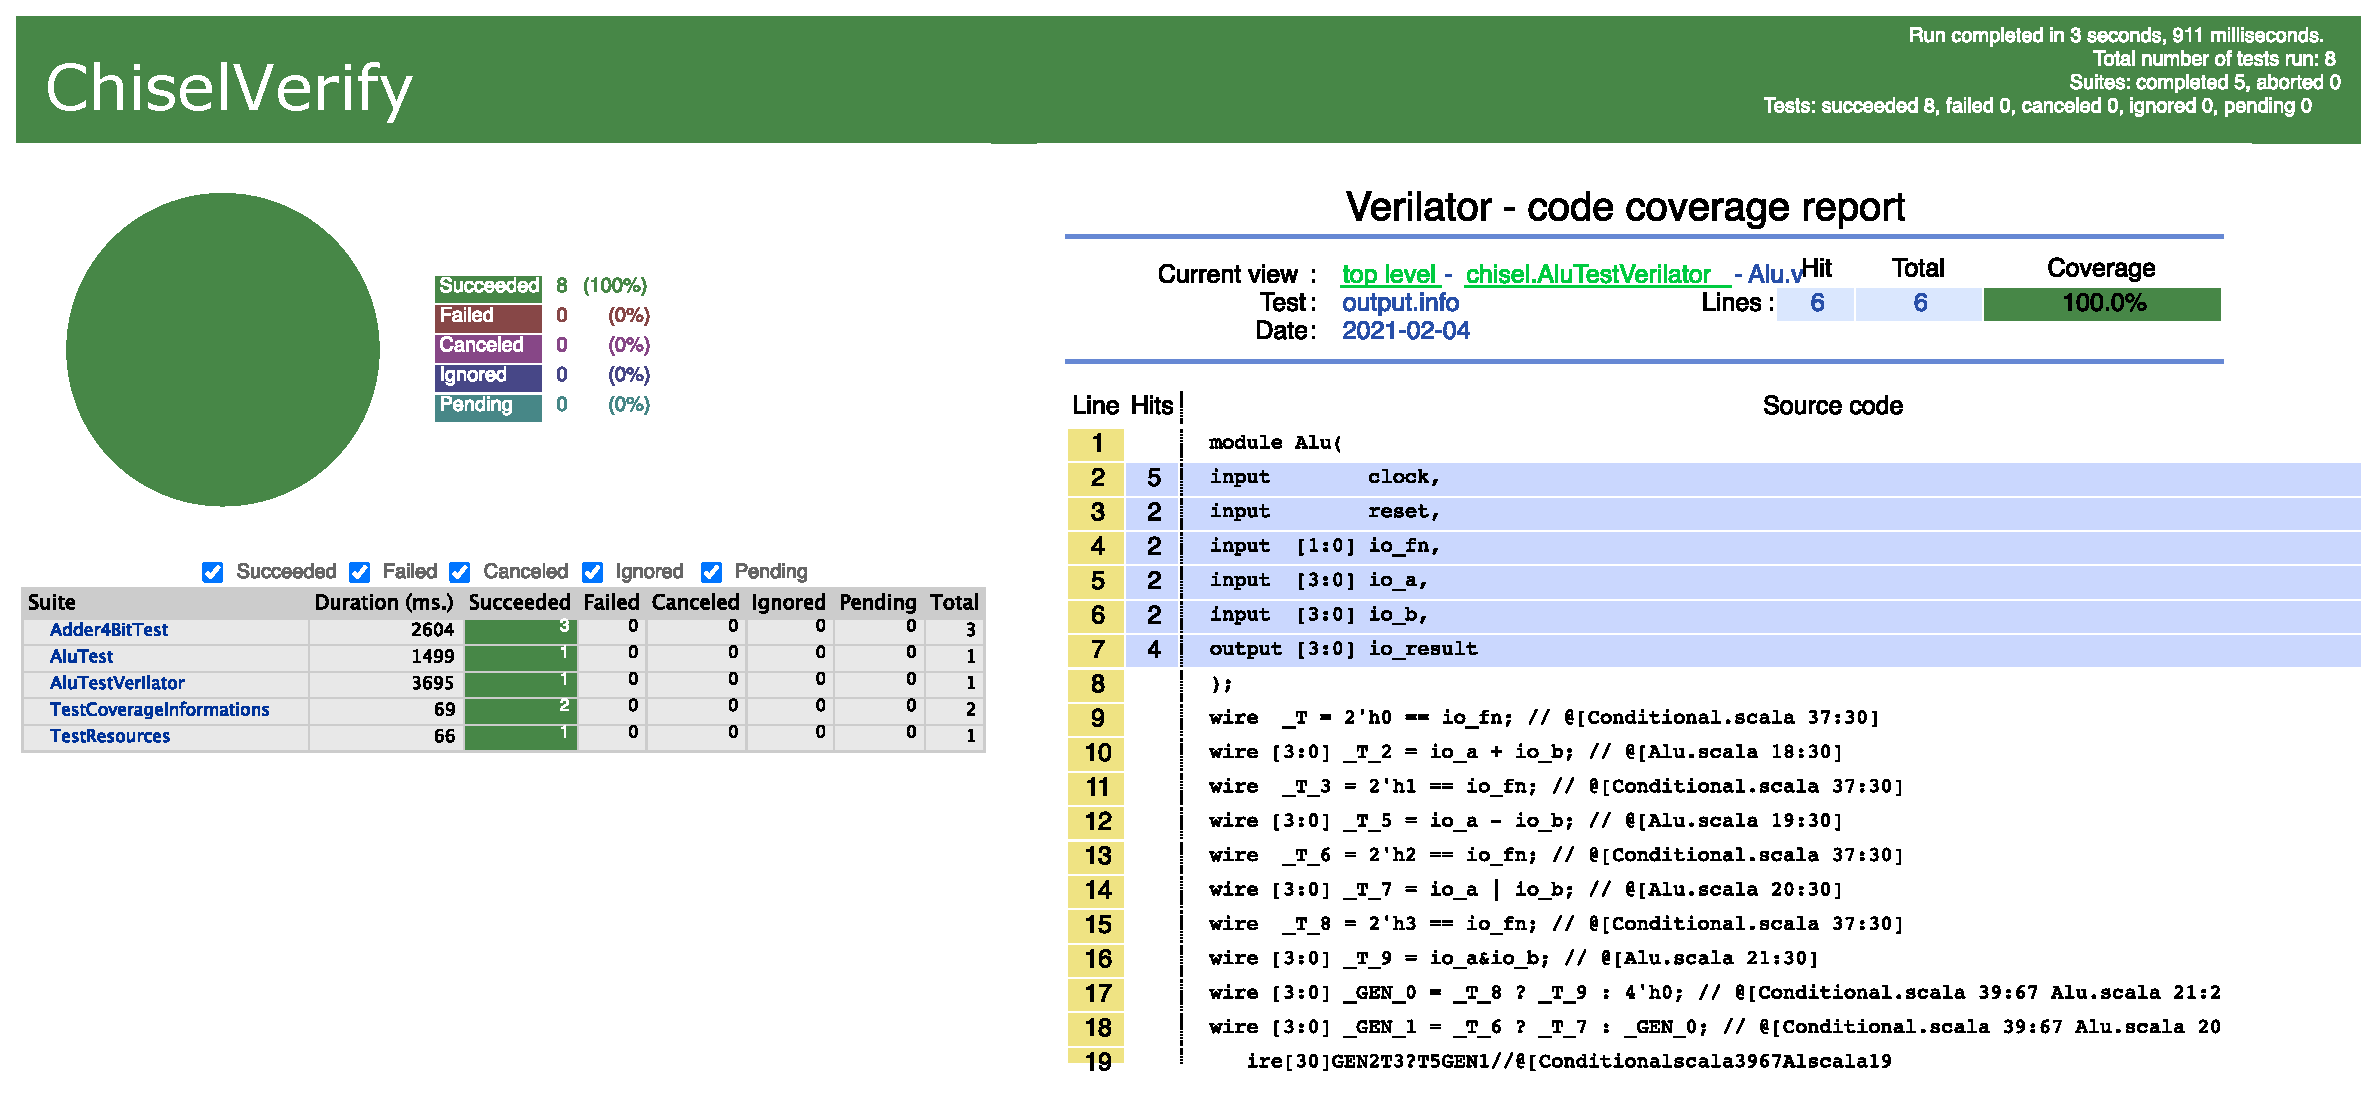
\includegraphics[width=\linewidth]{pictures/Chiselverify_html.eps}
\caption{Custom HTML ChiselTest report with Verilator coverage.}
\label{fig:customhtmlreport}
\end{figure}

Besides generating a code coverage report, the library also generates a table
containing all the functional coverage probes inserted in the test suite
displayed in figure \ref{fig:functionalcoveragebins}. This project was not
integrated into ``chiselverify" and is located in \cite{github:coverage}. From
the author's perspective, tools like the presented here are essential for
hardware verification because they facilitate the discovery of bugs and holes in
the verification process and are easily accessible by designers and verification
engineers.


\begin{figure}[!ht]
\centering
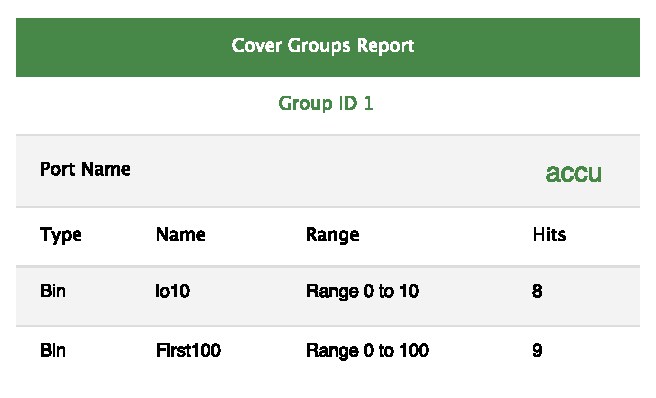
\includegraphics[width=0.4\linewidth]{pictures/Coverage_table.eps}
\caption{Functional Coverage table produced at the end of the test suite.}
\label{fig:functionalcoveragebins}
\end{figure}
